\index{Fourier transform}
\chapter{Fourier Transform}
\newthought{Decomposing Signals into Frequencies}


% ==============================================================================================
% INTRODUCTION BLOCK

\section{The Why}
\index{Fourier transform!motivation}

\newthought{In the previous chapters,} we represented functions by their values at sample points.
But many signals have underlying \emph{frequency} structure:
\begin{itemize}
    \item Audio: musical notes are combinations of frequencies
    \item Images: edges are high-frequency, smooth regions are low-frequency
    \item Time series: daily, weekly, yearly patterns
    \item Brain signals: alpha, beta, gamma waves at different frequencies
\end{itemize}

\newthought{The Fourier transform} decomposes any signal into a sum of sinusoids at different frequencies---revealing structure that's hidden in the time/space domain.

\marginnote{\newthought{Jean-Baptiste Joseph Fourier} (1768--1830) developed this theory while studying heat conduction. His claim that \emph{any} function could be represented as a sum of sines and cosines was initially controversial---even Lagrange objected!}

\index{frequency domain}
\newthought{Why frequency matters:}
\begin{itemize}
    \item \textbf{Compression:} Most signal energy is in few frequencies (MP3, JPEG)
    \item \textbf{Filtering:} Remove noise by cutting high frequencies
    \item \textbf{Analysis:} Identify periodic patterns (heart rhythms, stock cycles)
    \item \textbf{Computation:} Convolution is faster in frequency domain
\end{itemize}

\newthought{In machine learning and artificial intelligence:}
\begin{itemize}
    \item \textbf{Positional encoding:} Transformers use $\sin/\cos$ at different frequencies to encode position
    \item \textbf{Fourier features:} NeRF, SIREN use $\sin(\mathbf{W}\mathbf{x})$ to capture high-frequency detail
    \item \textbf{Spectral normalization:} GANs constrain Lipschitz constant via singular values
    \item \textbf{FFT convolution:} Efficient convolution in frequency domain for long sequences
    \item \textbf{Audio ML:} Speech recognition operates on spectrograms (time-frequency representations)
\end{itemize}

\newthought{Key insight:} Some patterns are easier to see in the frequency domain than in the time/space domain.
A noisy signal with a hidden periodic component becomes obvious when viewed as frequencies.



\newpage
\subsection{Hands On Experience}
\index{sinusoid}

\newthought{Consider the signal:}
\begin{equation}
    f(t) = \sin(2\pi t) + 0.5\sin(6\pi t)
\end{equation}

This is a sum of two pure frequencies: 1 Hz and 3 Hz.

\begin{figure}[h]
    \centering
    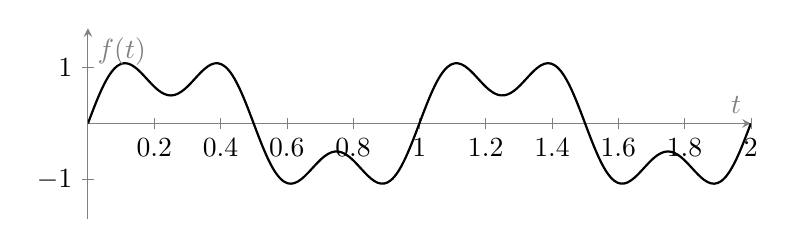
\begin{tikzpicture}
        \begin{axis}[
            width=10cm,
            height=4cm,
            axis x line=middle,
            axis y line=middle,
            xlabel={$t$},
            ylabel={$f(t)$},
            xmin=0, xmax=2,
            ymin=-1.7, ymax=1.7,
            tick style={gray},
            label style={gray},
            axis line style={gray},
        ]
        \addplot[black, thick, smooth, domain=0:2, samples=200] {sin(deg(2*3.14159*x)) + 0.5*sin(deg(6*3.14159*x))};
        \end{axis}
    \end{tikzpicture}
    \caption{A signal that's the sum of two sinusoids. Can you identify both frequencies by eye?}
    \label{fig:composite_signal}
\end{figure}

\newthought{In the time domain,} it's hard to tell what frequencies are present. The signal looks like a wobbly sine wave. But the Fourier transform reveals the truth: two spikes at 1 Hz (amplitude 1) and 3 Hz (amplitude 0.5).

\marginnote{\newthought{Time vs. Frequency:}
\begin{itemize}
    \item Time domain: \emph{when} things happen
    \item Frequency domain: \emph{what patterns} repeat
\end{itemize}
Both views contain the same information---just organized differently.}

\begin{figure}[h]
    \centering
    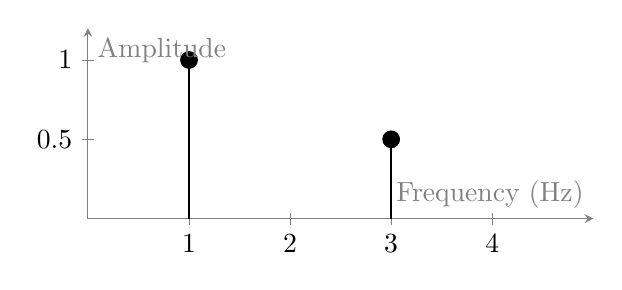
\begin{tikzpicture}
        \begin{axis}[
            width=8cm,
            height=4cm,
            axis x line=middle,
            axis y line=middle,
            xlabel={Frequency (Hz)},
            ylabel={Amplitude},
            xmin=0, xmax=5,
            ymin=0, ymax=1.2,
            tick style={gray},
            label style={gray},
            axis line style={gray},
            xtick={1, 2, 3, 4},
        ]
        % Frequency spikes
        \addplot[black, thick] coordinates {(1, 0) (1, 1)};
        \addplot[black, thick] coordinates {(3, 0) (3, 0.5)};
        \addplot[black, only marks, mark=*, mark size=3pt] coordinates {(1, 1) (3, 0.5)};
        \end{axis}
    \end{tikzpicture}
    \caption{Frequency spectrum of $f(t)$: clear spikes at 1 Hz and 3 Hz reveal the component frequencies.}
    \label{fig:frequency_spectrum}
\end{figure}

\vspace{1em}
\newthought{Why this matters for ML:} The transformer's positional encoding uses exactly this idea---encode position as a combination of sinusoids at different frequencies:
\begin{align}
    \text{PE}(\text{pos}, 2i) &= \sin(\text{pos} / 10000^{2i/d}) \\
    \text{PE}(\text{pos}, 2i+1) &= \cos(\text{pos} / 10000^{2i/d})
\end{align}

\marginnote{\newthought{Why multiple frequencies?} Low frequencies capture coarse position (beginning vs. end of sequence), high frequencies capture fine position (adjacent tokens). The combination encodes position at all scales simultaneously.}


\vspace{2em}
\newthought{The Learning Objectives} of this chapter aim at providing you with the abilities to:
\begin{itemize}
    \item Understand Fourier series representation of periodic functions
    \item Compute Fourier coefficients by hand for simple functions
    \item Compute and interpret the Discrete Fourier Transform (DFT)
    \item Apply the Fast Fourier Transform (FFT) algorithm
    \item Use the convolution theorem for efficient computation
    \item Connect Fourier features to positional encoding in transformers
\end{itemize}




% ==============================================================================================
% MAIN THEORY BLOCK

\newpage
\section{Fourier Series}
\index{Fourier series}

\newthought{Any periodic function} can be written as a sum of sines and cosines:

\begin{equation}
    \boxed{f(x) = \frac{a_0}{2} + \sum_{n=1}^{\infty} \left[a_n \cos(nx) + b_n \sin(nx)\right]}
\end{equation}

where the coefficients are computed as:
\begin{align}
    a_0 &= \frac{1}{\pi} \int_{-\pi}^{\pi} f(x) \, dx \quad \text{(average value)} \\
    a_n &= \frac{1}{\pi} \int_{-\pi}^{\pi} f(x) \cos(nx) \, dx \quad \text{(cosine coefficients)} \\
    b_n &= \frac{1}{\pi} \int_{-\pi}^{\pi} f(x) \sin(nx) \, dx \quad \text{(sine coefficients)}
\end{align}

\newthought{Intuition:} The coefficients $a_n, b_n$ measure ``how much'' of frequency $n$ is present in $f$.
Computing $a_n$ is like asking: ``How similar is $f$ to $\cos(nx)$?''

\marginnote{\newthought{Orthogonality:} The key property making this work is that sines and cosines at different frequencies are orthogonal:
\begin{align*}
    \int_{-\pi}^{\pi} \sin(nx)\sin(mx)\,dx &= 0 \text{ for } n \neq m \\
    \int_{-\pi}^{\pi} \cos(nx)\cos(mx)\,dx &= 0 \text{ for } n \neq m \\
    \int_{-\pi}^{\pi} \sin(nx)\cos(mx)\,dx &= 0 \text{ always}
\end{align*}
This orthogonality allows us to extract each coefficient independently.}


\subsection{Example: Square Wave}
\index{square wave}

\newthought{Consider the square wave:}
\begin{equation}
    f(x) = \begin{cases} 1 & 0 < x < \pi \\ -1 & -\pi < x < 0 \end{cases}
\end{equation}

\newthought{Computing coefficients:}

Since $f(x)$ is an odd function ($f(-x) = -f(x)$), all $a_n = 0$.

For $b_n$:
\begin{align*}
    b_n &= \frac{1}{\pi} \int_{-\pi}^{\pi} f(x) \sin(nx) \, dx \\
    &= \frac{2}{\pi} \int_{0}^{\pi} \sin(nx) \, dx \quad \text{(using symmetry)} \\
    &= \frac{2}{\pi} \left[-\frac{\cos(nx)}{n}\right]_0^{\pi} \\
    &= \frac{2}{\pi n} (1 - \cos(n\pi)) \\
    &= \begin{cases} \frac{4}{\pi n} & n \text{ odd} \\ 0 & n \text{ even} \end{cases}
\end{align*}

\newthought{Fourier series:}
\begin{equation}
    f(x) = \frac{4}{\pi}\left[\sin(x) + \frac{\sin(3x)}{3} + \frac{\sin(5x)}{5} + \frac{\sin(7x)}{7} + \cdots\right]
\end{equation}

Only odd harmonics appear (by symmetry of the square wave).

\begin{figure}[h]
    \centering
    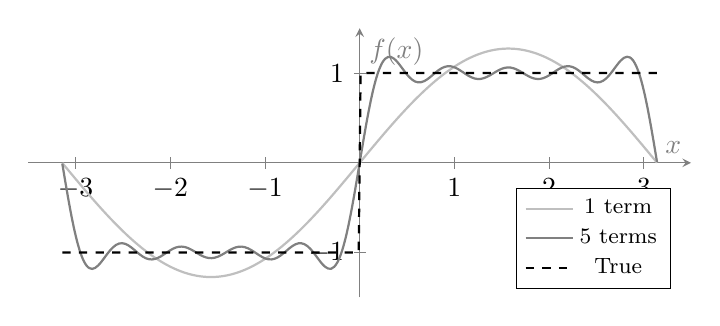
\begin{tikzpicture}
        \begin{axis}[
            width=10cm,
            height=5cm,
            axis x line=middle,
            axis y line=middle,
            xlabel={$x$},
            ylabel={$f(x)$},
            xmin=-3.5, xmax=3.5,
            ymin=-1.5, ymax=1.5,
            tick style={gray},
            label style={gray},
            axis line style={gray},
            legend pos=south east,
            legend style={font=\footnotesize},
        ]
        % 1 term
        \addplot[gray!50, thick, smooth, domain=-3.14:3.14, samples=100]
            {4/3.14159*sin(deg(x))};
        \addlegendentry{1 term}
        % 5 terms
        \addplot[gray, thick, smooth, domain=-3.14:3.14, samples=200]
            {4/3.14159*(sin(deg(x)) + sin(deg(3*x))/3 + sin(deg(5*x))/5 + sin(deg(7*x))/7 + sin(deg(9*x))/9)};
        \addlegendentry{5 terms}
        % True square wave
        \addplot[black, dashed, thick] coordinates {(-3.14, -1) (-0.01, -1) (0.01, 1) (3.14, 1)};
        \addlegendentry{True}
        \end{axis}
    \end{tikzpicture}
    \caption{Fourier series approximation of square wave. More terms give closer approximation, but the ``Gibbs phenomenon'' causes overshoot at discontinuities.}
    \label{fig:square_wave_fourier}
\end{figure}

\marginnote{\newthought{Gibbs phenomenon:} Near discontinuities, the Fourier series always overshoots by about 9\%, no matter how many terms you use. This is a fundamental limitation, not a bug.}




\newpage
\section{Discrete Fourier Transform}
\index{Discrete Fourier Transform}
\index{DFT}

\newthought{For sampled data,} we use the Discrete Fourier Transform (DFT).

Given $N$ samples $x_0, x_1, \ldots, x_{N-1}$, the DFT is:

\begin{equation}
    \boxed{X_k = \sum_{n=0}^{N-1} x_n \cdot e^{-2\pi i kn/N}, \quad k = 0, 1, \ldots, N-1}
\end{equation}

\newthought{Interpretation:}
\begin{itemize}
    \item $X_k$ = complex amplitude at frequency $k$
    \item $|X_k|$ = magnitude (how much of frequency $k$)
    \item $\arg(X_k)$ = phase (where in the cycle the frequency starts)
    \item $k = 0$: DC component (average value)
    \item $k = N/2$: Nyquist frequency (highest representable)
\end{itemize}

\marginnote{\newthought{Euler's formula:} $e^{i\theta} = \cos\theta + i\sin\theta$. The complex exponential elegantly encodes both sine and cosine components in one number.}

\newthought{Inverse DFT:}
\begin{equation}
    x_n = \frac{1}{N} \sum_{k=0}^{N-1} X_k \cdot e^{2\pi i kn/N}
\end{equation}

The signal can be perfectly reconstructed from its frequency components---no information is lost!


\subsection{Example: DFT by Hand}
\index{DFT!example}

\newthought{Compute the DFT of $x = [1, 0, -1, 0]$} (N = 4).

The twiddle factor is $W_4 = e^{-2\pi i/4} = e^{-i\pi/2} = -i$.

Powers: $W_4^0 = 1$, $W_4^1 = -i$, $W_4^2 = -1$, $W_4^3 = i$.

\begin{align*}
    X_0 &= x_0 W_4^0 + x_1 W_4^0 + x_2 W_4^0 + x_3 W_4^0 \\
    &= 1 \cdot 1 + 0 \cdot 1 + (-1) \cdot 1 + 0 \cdot 1 = 0 \quad \text{(DC = 0, average is zero)} \\[0.5em]
    X_1 &= x_0 W_4^0 + x_1 W_4^1 + x_2 W_4^2 + x_3 W_4^3 \\
    &= 1 \cdot 1 + 0 \cdot (-i) + (-1) \cdot (-1) + 0 \cdot i = 1 + 1 = 2 \\[0.5em]
    X_2 &= x_0 W_4^0 + x_1 W_4^2 + x_2 W_4^4 + x_3 W_4^6 \\
    &= 1 \cdot 1 + 0 \cdot (-1) + (-1) \cdot 1 + 0 \cdot (-1) = 0 \\[0.5em]
    X_3 &= x_0 W_4^0 + x_1 W_4^3 + x_2 W_4^6 + x_3 W_4^9 \\
    &= 1 \cdot 1 + 0 \cdot i + (-1) \cdot (-1) + 0 \cdot (-i) = 2
\end{align*}

\marginnote{\newthought{Result:} $X = [0, 2, 0, 2]$. Energy at frequencies 1 and 3 (which is $N-1$, the alias of frequency 1). The signal $[1, 0, -1, 0]$ oscillates at the fundamental frequency.}

\newthought{Result:} $X = [0, 2, 0, 2]$.

The signal has energy at frequencies 1 and 3. Note that $X_3 = X_1^*$ (complex conjugate)---this symmetry always holds for real signals.




\newpage
\section{Fast Fourier Transform}
\index{Fast Fourier Transform}
\index{FFT}
\index{Cooley-Tukey}

\newthought{The problem:} Naive DFT computation costs $O(N^2)$ operations (N outputs, each summing N terms).

\newthought{The solution:} The Cooley-Tukey FFT algorithm computes the DFT in $O(N \log N)$.

\newthought{Key idea:} Divide and conquer. Split the DFT into two half-size DFTs by separating even and odd indices.

Let $W_N = e^{-2\pi i/N}$. Then:
\begin{align}
    X_k &= \sum_{n=0}^{N-1} x_n W_N^{kn} \\
    &= \underbrace{\sum_{m=0}^{N/2-1} x_{2m} W_N^{k(2m)}}_{\text{even indices}} + \underbrace{\sum_{m=0}^{N/2-1} x_{2m+1} W_N^{k(2m+1)}}_{\text{odd indices}} \\
    &= \sum_{m=0}^{N/2-1} x_{2m} W_{N/2}^{km} + W_N^k \sum_{m=0}^{N/2-1} x_{2m+1} W_{N/2}^{km}
\end{align}

\begin{equation}
    \boxed{X_k = E_k + W_N^k \cdot O_k}
\end{equation}

where $E_k$ is the DFT of even-indexed samples and $O_k$ is the DFT of odd-indexed samples.

\marginnote{\newthought{Recursion:}
\begin{itemize}
    \item Size-$N$ DFT $\to$ two size-$N/2$ DFTs
    \item Each size-$N/2$ $\to$ two size-$N/4$ DFTs
    \item Continue until size 1
    \item Depth: $\log_2 N$ levels
    \item Work per level: $O(N)$
    \item Total: $O(N \log N)$
\end{itemize}}

\newthought{Complexity comparison:}
\begin{table*}[ht]
\centering
\begin{tabular}{p{0.20\textwidth}p{0.25\textwidth}p{0.25\textwidth}}
\toprule
\textbf{Algorithm} & \textbf{Operations} & \textbf{For $N = 10^6$} \\
\midrule
Naive DFT & $O(N^2)$ & $10^{12}$ \\
FFT & $O(N \log N)$ & $2 \times 10^7$ \\
\bottomrule
\end{tabular}
\vspace{2em}
\caption{FFT reduces DFT computation from $O(N^2)$ to $O(N \log N)$, a 50,000$\times$ speedup for $N = 10^6$.}
\label{tab:fft_complexity}
\end{table*}

FFT is 50,000$\times$ faster for $N = 10^6$!

\begin{figure}[h]
    \centering
    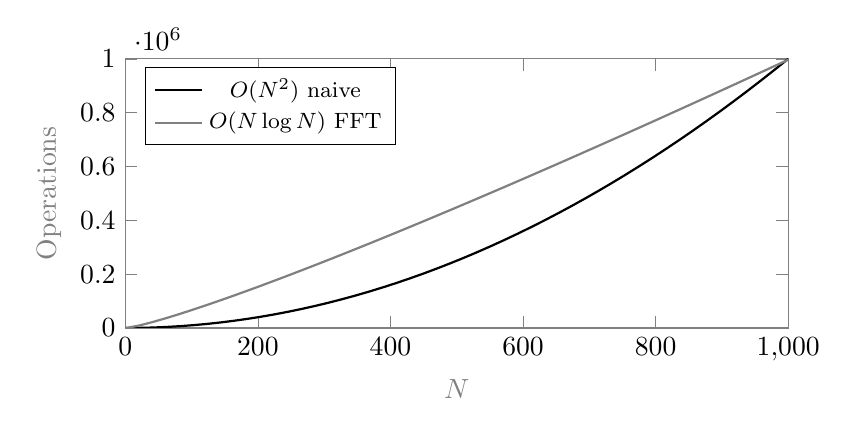
\begin{tikzpicture}
        \begin{axis}[
            width=10cm,
            height=5cm,
            xlabel={$N$},
            ylabel={Operations},
            xmin=0, xmax=1000,
            ymin=0, ymax=1e6,
            tick style={gray},
            label style={gray},
            axis line style={gray},
            legend pos=north west,
            legend style={font=\footnotesize},
        ]
        \addplot[black, thick, domain=1:1000, samples=50] {x^2};
        \addlegendentry{$O(N^2)$ naive}
        \addplot[gray, thick, domain=1:1000, samples=50] {x*ln(x)/ln(2)*100};
        \addlegendentry{$O(N \log N)$ FFT}
        \end{axis}
    \end{tikzpicture}
    \caption{FFT complexity vs. naive DFT. The difference grows dramatically with $N$.}
    \label{fig:fft_complexity}
\end{figure}

\newthought{Practical impact of FFT:}
\begin{itemize}
    \item Real-time audio processing (MP3, AAC encoding/decoding)
    \item Image compression (JPEG uses DCT, a variant)
    \item Efficient convolution in signal processing and some CNNs
    \item Spectral analysis in scientific computing
    \item Polynomial multiplication in cryptography
\end{itemize}




\newpage
\section{Convolution Theorem}
\index{convolution theorem}
\index{convolution}

\newthought{Convolution in time} corresponds to \textbf{multiplication in frequency}:

\begin{equation}
    \boxed{\mathcal{F}\{f * g\} = \mathcal{F}\{f\} \cdot \mathcal{F}\{g\}}
\end{equation}

where $*$ denotes convolution: $(f * g)(t) = \int f(\tau) g(t - \tau) d\tau$

and $\cdot$ is element-wise multiplication.

\marginnote{\newthought{Duality:} The converse is also true: multiplication in time becomes convolution in frequency. This duality is one of the beautiful symmetries of Fourier analysis.}

\newthought{Why this matters:}
\begin{itemize}
    \item Direct convolution: $O(N^2)$ operations
    \item FFT convolution: $O(N \log N)$ operations
\end{itemize}

\newthought{Fast convolution algorithm:}
\begin{enumerate}
    \item Zero-pad both signals to length $N \geq |f| + |g| - 1$
    \item Compute FFT of both: $F = \text{FFT}(f)$, $G = \text{FFT}(g)$
    \item Multiply element-wise: $H = F \cdot G$
    \item Inverse FFT: $h = \text{IFFT}(H)$
\end{enumerate}

Total cost: $3 \times O(N \log N) = O(N \log N)$, much better than $O(N^2)$.

\newthought{Example:} Convolve $f = [1, 2, 3]$ with $g = [1, 1]$.

Direct: $(f * g)_0 = 1 \cdot 1 = 1$, $(f * g)_1 = 1 \cdot 1 + 2 \cdot 1 = 3$, $(f * g)_2 = 2 \cdot 1 + 3 \cdot 1 = 5$, $(f * g)_3 = 3 \cdot 1 = 3$.

Result: $[1, 3, 5, 3]$.

\marginnote{\newthought{In CNNs,} convolution is the core operation. For small kernels (3$\times$3), direct convolution with CUDA optimization is faster. For large kernels or long sequences (audio, time series), FFT convolution wins.}


\subsection{Filtering}
\index{filtering}

\newthought{Frequency-domain filtering:} Modify specific frequencies.

\begin{itemize}
    \item \textbf{Low-pass filter:} Keep low frequencies, remove high (smoothing)
    \item \textbf{High-pass filter:} Keep high frequencies, remove low (edge detection)
    \item \textbf{Band-pass filter:} Keep frequencies in a range (isolate a signal)
\end{itemize}

This is how noise reduction works: noise is typically high-frequency, so a low-pass filter removes it while preserving the signal.




\newpage
\section{Fourier Features in Deep Learning}
\index{Fourier features}
\index{positional encoding}

\newthought{Neural networks struggle} with high-frequency functions. A standard MLP trying to learn $\sin(100x)$ needs many layers and still produces blurry results.

\newthought{The spectral bias:} Neural networks have an inductive bias toward learning low-frequency functions first. High-frequency details are learned slowly or not at all.

\marginnote{\newthought{Why spectral bias?} The gradient flow in neural networks favors smooth functions. Sharp variations require precise weight configurations that are hard to find via gradient descent.}

\newthought{Fourier feature mapping:} Transform inputs through sinusoids before the network:
\begin{equation}
    \gamma(\mathbf{x}) = [\cos(2\pi \mathbf{B} \mathbf{x}), \sin(2\pi \mathbf{B} \mathbf{x})]
\end{equation}

where $\mathbf{B}$ is a matrix of frequency vectors.

This allows networks to learn high-frequency functions easily!


\subsection{Transformer Positional Encoding}
\index{positional encoding!transformer}

\newthought{The transformer architecture} has no built-in notion of position---it treats input as a set. Positional encoding adds position information:

\begin{align}
    \text{PE}(\text{pos}, 2i) &= \sin\left(\text{pos} / 10000^{2i/d_{\text{model}}}\right) \\
    \text{PE}(\text{pos}, 2i+1) &= \cos\left(\text{pos} / 10000^{2i/d_{\text{model}}}\right)
\end{align}

\newthought{Why this specific form?}
\begin{itemize}
    \item \textbf{Unique encoding:} Each position gets a unique vector
    \item \textbf{Bounded values:} Sine/cosine stay in $[-1, 1]$
    \item \textbf{Relative positions:} $\text{PE}(\text{pos} + k)$ can be expressed as a linear function of $\text{PE}(\text{pos})$
    \item \textbf{Smooth interpolation:} Works for positions longer than training
\end{itemize}

\marginnote{\newthought{Frequency range:}
\begin{itemize}
    \item $i = 0$: wavelength $= 2\pi$ (distinguishes adjacent positions)
    \item $i = d/2$: wavelength $= 2\pi \cdot 10000$ (distinguishes sequence start from end)
\end{itemize}
The geometric progression covers all scales.}


\subsection{NeRF and SIREN}
\index{NeRF}
\index{SIREN}

\newthought{Neural Radiance Fields (NeRF)} use Fourier features to represent 3D scenes with fine detail:
\begin{equation}
    \gamma(p) = [\sin(2^0 \pi p), \cos(2^0 \pi p), \ldots, \sin(2^{L-1} \pi p), \cos(2^{L-1} \pi p)]
\end{equation}

Without Fourier features, NeRF produces blurry images. With them, it captures sharp edges and fine textures.

\newthought{SIREN} (Sinusoidal Representation Networks) use $\sin$ as the activation function throughout:
\begin{equation}
    \phi(\mathbf{x}) = \sin(\mathbf{W}\mathbf{x} + \mathbf{b})
\end{equation}

This enables learning signals with complex frequency content, including images, audio, and 3D shapes.




% ==============================================================================================
% STUDENT ACTIVATION BLOCK

\newpage
\section{Examples \& Exercises}
\index{Fourier transform!exercises}

\marginnote{\newthought{Code} can be found at \url{https://github.com/Quillstacks/lecturecode_numericalmethods.git}.}

\newthought{Exercise 1: Fourier coefficients.} Compute the Fourier coefficients for $f(x) = x$ on $[-\pi, \pi]$.

\textit{Hint:} $f(x) = x$ is an odd function, so $a_n = 0$ for all $n$.

For $b_n$, integrate by parts:
\begin{align*}
    b_n &= \frac{1}{\pi} \int_{-\pi}^{\pi} x \sin(nx) \, dx = \frac{2}{\pi} \int_0^{\pi} x \sin(nx) \, dx \\
    &= \frac{2}{\pi} \left[-\frac{x \cos(nx)}{n} + \frac{\sin(nx)}{n^2}\right]_0^{\pi} = \frac{2(-1)^{n+1}}{n}
\end{align*}

So $f(x) = 2\left[\sin(x) - \frac{\sin(2x)}{2} + \frac{\sin(3x)}{3} - \cdots\right]$.


\vspace{2em}
\newthought{Exercise 2: 4-point DFT.} Compute the DFT of $x = [1, 1, 1, 1]$.

\textit{Solution:}
\begin{align*}
    X_0 &= 1 + 1 + 1 + 1 = 4 \\
    X_1 &= 1 + 1 \cdot (-i) + 1 \cdot (-1) + 1 \cdot (i) = 1 - i - 1 + i = 0 \\
    X_2 &= 1 + 1 \cdot (-1) + 1 \cdot (1) + 1 \cdot (-1) = 0 \\
    X_3 &= 1 + 1 \cdot (i) + 1 \cdot (-1) + 1 \cdot (-i) = 0
\end{align*}

All energy is in $X_0$ (DC component)---a constant signal has only zero frequency.


\vspace{2em}
\newthought{Exercise 3: Frequency identification.} An audio signal sampled at 44.1 kHz has FFT peak at index $k = 1000$ out of $N = 44100$ samples.

What frequency (in Hz) does this correspond to?

\textit{Solution:} Frequency $f = k \cdot f_s / N = 1000 \times 44100 / 44100 = 1000$ Hz.

This is the note B5 (approximately).


\vspace{2em}
\newthought{Exercise 4: Positional encoding.} For $d_{\text{model}} = 4$ and position $\text{pos} = 3$:
\begin{enumerate}
    \item Compute all 4 components of the positional encoding
    \item How does it differ from position 4?
    \item Why use both sine and cosine?
\end{enumerate}

\textit{Solution:}
\begin{align*}
    \text{PE}(3, 0) &= \sin(3 / 10000^{0/4}) = \sin(3) \approx 0.14 \\
    \text{PE}(3, 1) &= \cos(3 / 10000^{0/4}) = \cos(3) \approx -0.99 \\
    \text{PE}(3, 2) &= \sin(3 / 10000^{2/4}) = \sin(0.03) \approx 0.03 \\
    \text{PE}(3, 3) &= \cos(3 / 10000^{2/4}) = \cos(0.03) \approx 1.00
\end{align*}




\newpage
\section{Self-Reflection and Recap}
\index{Fourier transform!recap}

\newthought{Self-Reflection} Questions to guide your understanding:
\begin{itemize}
    \item Why does the transformer use multiple frequencies in positional encoding?
    \item What does ``high frequency'' mean for images? For audio?
    \item Why is FFT crucial for efficient long-sequence models?
    \item How does the convolution theorem speed up signal processing?
    \item What information is in the phase vs. magnitude of the DFT?
    \item Why do neural networks have spectral bias toward low frequencies?
\end{itemize}

\newthought{Recap} of Key Concepts:
\begin{itemize}
    \item \textbf{Fourier series:} Decompose periodic functions into sines and cosines; coefficients measure frequency content.
    \item \textbf{DFT:} Discrete version for sampled data; $X_k$ = complex amplitude at frequency $k$.
    \item \textbf{FFT:} $O(N \log N)$ algorithm using divide-and-conquer---essential for practical applications.
    \item \textbf{Convolution theorem:} Convolution in time = multiplication in frequency; enables fast filtering.
    \item \textbf{Fourier features:} Help neural networks learn high-frequency functions; used in positional encoding, NeRF, SIREN.
\end{itemize}


\marginnote{\newthought{Teaser.} Fourier analysis shows what frequencies exist in a signal---a static view. But many systems \textbf{evolve over time}: populations grow, objects move, neurons fire. How do we model \textbf{dynamics}?}

\newthought{From frequency to dynamics.} The Fourier transform analyzes signals but doesn't model how systems change over time. In the next chapter, we'll study \emph{differential equations}---the mathematical language of dynamics---and see how ResNets are actually Euler steps for solving ODEs.



%%%%%%%%%%%%%%%%%%%%%%%%%%%%%%%%%%%%%%%%%%%%%%%%%%%%%%%%%%%%%%%%%%%%%%%%%%%%%%
